\documentclass[tikz,svgnames]{standalone}

\usetikzlibrary{decorations.pathmorphing}

\begin{document}
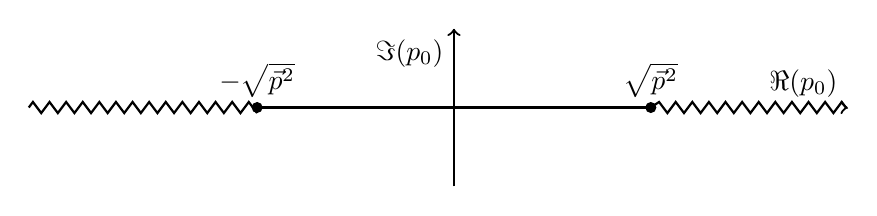
\begin{tikzpicture}[thick]

  \def\xr{5} \def\yr{1}

  % Labels
  \fill (-\xr/2,0) circle (2pt) node[above] (leftbranch) {$-\sqrt{\vec{p}^2}$} (\xr/2,0) circle (2pt) node[above] (rightbranch) {$\sqrt{\vec{p}^2}$};

  % Axes
  \draw [->,decorate,decoration={zigzag,segment length=6,amplitude=2}] (-\xr-0.4,0) -- (leftbranch.south) (rightbranch.south) -- (\xr,0) node [above left]  {$\Re(p_0)$};
  \draw (leftbranch.south) -- (rightbranch.south);
  \draw [->] (0,-\yr) -- (0,\yr) node[below left=0.1] {$\Im(p_0)$};

\end{tikzpicture}
\end{document}